\documentclass[conference,a4paper]{IEEEtran}
\usepackage{cite}
\usepackage{amsmath}
\usepackage{graphicx}
\usepackage{booktabs}
\usepackage{array}
\usepackage[hidelinks]{hyperref}
\usepackage{xurl}
\emergencystretch=1em
\begin{document}
\title{Enterprise AI Systems with MCP-Swarm: A Rotational Multi-Agent Framework for Persistent Memory, Consensus Reasoning, and Intelligent Document Understanding}
\author{\IEEEauthorblockN{Venu Kalluru}
\IEEEauthorblockA{\textit{Independent Researcher}\\
Cumming, Georgia, USA\\
vmvk04@gmail.com}}
\maketitle
\begin{abstract}
Enterprise assistants built on large language models (LLMs) must call tools safely, decide when to trust an answer and carry knowledge across sessions. MCP-Swarm combines a Model Context Protocol (MCP) gateway with task-scoped tokens, a rotational council that queries four of seven models and merges their answers by confidence and agreement, and a persistent memory that is retrieved only above a similarity threshold. This paper evaluates the design with a controlled, reproducible protocol. Seven open-weight models of 1--1.7 billion parameters answered 300 questions from the Massive Multitask Language Understanding (MMLU) benchmark on a CPU, and single-model, fixed, rotational and random councils were compared on the same outputs over ten seeds with exact paired tests. No council beat the best single model: the rotational council reached 44.6\% against 57.7\% at four times the token cost, because near-chance members outvoted the strongest one. Rotation matched random selection in accuracy and bounded model idle time; confidence carried more signal than agreement. In a synthetic multi-session memory task, threshold-gated retrieval answered all 68 stored-fact queries at 102 prompt tokens per query, against 79.4\% at 2,137 tokens for full history, and withheld memory from 29 of 32 queries that needed none. In a small real MCP run, no unauthorised export call succeeded. The results support adaptive memory and gateway controls, and show that equal-weight councils need strong, comparable members to pay for their cost.
\end{abstract}
\begin{IEEEkeywords}
Model Context Protocol, multi-agent systems, LLM ensembles, consensus, retrieval-augmented memory, tool authorization
\end{IEEEkeywords}
\begin{figure*}[t]
\centering
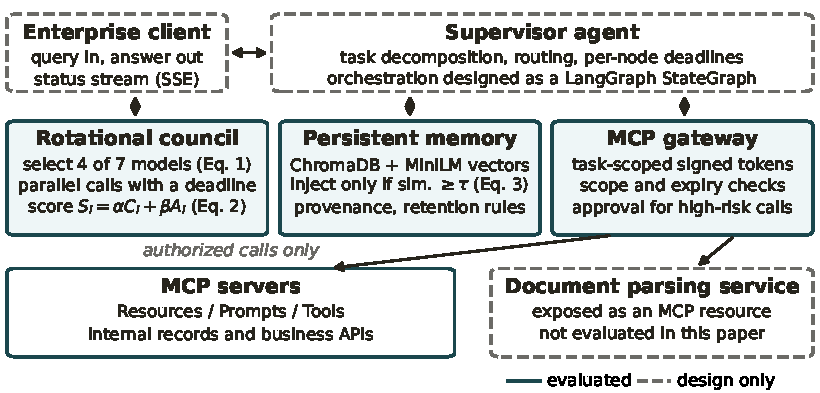
\includegraphics[width=0.94\textwidth]{figs/fig1_arch.pdf}
\caption{MCP-Swarm architecture. Solid borders mark components implemented and evaluated in this paper; dashed borders mark design components that were not evaluated. Arrows show request and response paths; tool calls reach MCP servers only through the gateway.}
\label{fig:arch}
\end{figure*}
\section{Introduction}
Enterprise assistants built on large language models (LLMs) now call tools, read internal records and keep state between sessions. Three engineering problems recur in such deployments. Tool integration is still largely bespoke, although the Model Context Protocol (MCP) now defines a common interface for resources, prompts and tools \cite{mcpspec}, and that interface brings its own attack surface \cite{hou2025mcp}. A single model answering alone gives no internal signal when it is wrong. Carrying a long conversation history into every prompt raises token cost and can bury the one relevant fact among irrelevant text.

MCP-Swarm addresses these problems with three cooperating components: an MCP gateway that admits only task-scoped tool calls, a rotational council that queries four of seven heterogeneous models and merges their answers, and a persistent memory that is consulted only when a stored entry is semantically close to the query. This paper evaluates the design with a controlled, repeatable protocol on public data and open-weight models, states the datasets, baselines and configurations used, and reports outcomes that do not favour the design as well as those that do.

The contributions are: (i) an architecture that states its trust boundaries and marks which parts are implemented and evaluated; (ii) a controlled comparison of single-model, fixed four-model, rotational and random councils on 300 public benchmark questions with ten rotation seeds, consensus-term ablations, and measured latency and token use; (iii) an experiment isolating adaptive memory activation against no memory, full history and fixed top-$k$ retrieval; and (iv) deadline, member-failure and tool-security results.

\section{Related Works}
Multi-agent LLM frameworks are surveyed by Guo et al.\ \cite{guo2024survey}. AutoGen \cite{wu2023autogen}, CAMEL \cite{li2023camel} and MetaGPT \cite{hong2023metagpt} coordinate role-specialised agents through conversation, and a study of failed multi-agent runs attributes many errors to specification and coordination faults rather than to model capacity \cite{cemri2025fail}. MCP-Swarm differs mainly in placing a protocol gateway and an explicit aggregation rule between agents and tools.

Aggregating several answers is a well-tested way to reduce error. Self-consistency samples one model repeatedly and takes the majority \cite{wang2023selfconsistency}; multi-agent debate lets models revise answers after reading one another \cite{du2024debate}; Mixture-of-Agents layers proposers and an aggregator \cite{wang2024moa}; LLM-Blender ranks and fuses candidates \cite{jiang2023blender}. Chen et al.\ show that accuracy does not rise monotonically with the number of calls and can fall on hard queries \cite{chen2024calls}. Classical ensemble theory explains why: gains depend on members whose errors are not strongly correlated \cite{dietterich2000ensemble}. Weighted synthesis also inherits the fault-tolerance question posed by the Byzantine generals problem \cite{lamport1982byzantine}. The rotational council is a small, cost-bounded variant of these ideas, and the evaluation below asks whether rotation adds anything beyond aggregation itself.

Retrieval-augmented generation (RAG) supplies retrieved passages at inference time \cite{lewis2020rag}, and MemGPT manages a tiered memory for long-running agents \cite{packer2023memgpt}. Long prompts are not free: models use information placed in the middle of a long context less reliably \cite{liu2024lost}. MCP-Swarm retrieves stored memories with sentence embeddings \cite{reimers2019sbert} and admits them only above a similarity threshold, so a query that needs no memory carries none. Indirect prompt injection through retrieved content \cite{greshake2023injection}, MCP-specific attacks catalogued by MCPSecBench \cite{yang2025mcpsecbench} and the OWASP risk list for LLM applications \cite{owasp2025} motivate the gateway and memory controls described next.

\section{Methods}
\subsection{Architecture}
Fig.~\ref{fig:arch} shows the components. The supervisor agent decomposes a request and routes sub-tasks; its orchestration is designed as a LangGraph state graph \cite{langgraph}, while the experiments below drive the council, memory and gateway directly from a Python harness. Components drawn with dashed borders, including the supervisor and a document-parsing service exposed as an MCP resource, are design elements that this paper does not evaluate.

\textit{Rotational council.} Seven models from seven developers form the pool. For each query four are drawn without replacement with probability
\begin{equation}
P(m) \propto w_m + \lambda\, g_m ,
\label{eq:rot}
\end{equation}
where $w_m=1$ is a base weight, $g_m$ is the number of queries since model $m$ was last selected and $\lambda=0.15$. The bonus spreads load and exposure across the pool. Each selected model returns an answer, and the answer with the highest score
\begin{equation}
S_i = \alpha C_i + \beta A_i ,\qquad \alpha=\beta=0.5,
\label{eq:score}
\end{equation}
is returned, where $C_i$ is model $i$'s normalised probability for its chosen option and $A_i$ is the fraction of the other council members that gave the same answer. A member that misses the deadline is dropped and the remaining members are scored.

\textit{Adaptive memory.} Memory entries from earlier sessions are embedded with all-MiniLM-L6-v2 and stored in ChromaDB \cite{chroma}. For a new query the five nearest entries are retrieved, and only those with cosine similarity
\begin{equation}
\mathrm{sim}(q,m)=\frac{\mathbf{v}_q\cdot\mathbf{v}_m}{\lVert\mathbf{v}_q\rVert\,\lVert\mathbf{v}_m\rVert}\ \geq\ \tau
\label{eq:sim}
\end{equation}
enter the prompt. Entries carry their source session, and retention rules can exclude classes of data from retrieval.

\textit{MCP gateway.} Every tool call carries a signed token bound to one task, a role and an expiry time. The gateway rejects calls outside the token's tool scope, calls that reuse another task's token, expired tokens and high-risk operations that lack supervisor approval. Content returned by tools or memory is passed to models as data in a separate channel, never as instructions.

\section{Results and Discussion}
\subsection{Experimental Setup}
\textit{Dataset.} The council was tested on 300 four-option questions from the test split of the Massive Multitask Language Understanding (MMLU) benchmark \cite{hendrycks2021mmlu}, 50 each from professional accounting and high-school macroeconomics (finance), jurisprudence and international law (law), and computer security and college computer science (technology). The questions were sampled once with a fixed seed (20261015) before any model was run, and none were used for tuning. Accuracy is the share of questions answered with the gold letter; chance is 25\%.

\textit{Models and runtime.} The pool contains seven instruction-tuned open-weight models of 1--1.7 billion parameters from seven developers (Table~\ref{tab:models}), each quantised to 4-bit (Q4\_K\_M) and served by llama.cpp \cite{llamacpp} on a 2-core CPU with 7\,GB of memory. Every call used temperature 0, one output token and the same prompt. $C_i$ in (\ref{eq:score}) is the model's probability for its chosen letter, renormalised over A--D from the top-20 token log-probabilities. Wall-clock latency and the token counts reported by the server were logged per call; prompt caching was disabled.

\textit{Configurations.} Each model answered every question once; council outcomes were then computed from these logged answers, so all configurations are compared on identical model outputs. The configurations are: the best single model; a round-robin single model (rotation without a council); all seven models; a fixed four-model council chosen a priori (the four largest models); the best of all 35 fixed four-model councils, selected on the test set and therefore optimistic; the rotational council of (\ref{eq:rot}) with four aggregation rules (Eq.~(\ref{eq:score}), plurality vote, confidence only and agreement only); and a uniformly random four-model council as the control for rotation. Rotational and random councils were run with ten seeds. Members were queried sequentially, so the parallel latency of a council is estimated as the slowest member's measured latency. Paired differences against the best single model use the exact McNemar test, and 95\% confidence intervals (CIs) use 10,000 bootstrap resamples of the questions.

\subsection{Single Models and Councils}
Table~\ref{tab:models} shows a wide spread in single-model accuracy. Qwen2.5-1.5B reached 57.7\%, Gemma-3-1B and Falcon3-1B about 43\%, and the other four models 28--29\%, close to chance. No call produced an invalid answer.

\begin{table}[t]
\caption{Single-Model Results on 300 MMLU Questions}
\label{tab:models}
\centering
\footnotesize
\setlength{\tabcolsep}{3.5pt}
\begin{tabular}{@{}lccccc@{}}
\toprule
Model & Acc. (\%) & 95\% CI & p50 (s) & p95 (s) & Tokens \\
\midrule
Qwen2.5-1.5B & 57.7 & 52.0--63.3 & 1.57 & 2.89 & 133 \\
Gemma-3-1B & 43.0 & 37.3--48.7 & 1.32 & 2.29 & 135 \\
Falcon3-1B & 42.7 & 37.0--48.3 & 1.42 & 2.26 & 144 \\
OLMo-2-1B & 28.7 & 23.7--34.0 & 1.25 & 1.98 & 134 \\
Llama-3.2-1B & 28.3 & 23.3--33.3 & 1.29 & 1.93 & 153 \\
SmolLM2-1.7B & 28.0 & 23.0--33.0 & 2.05 & 3.41 & 141 \\
Granite-3.1-1B & 27.7 & 22.7--32.7 & 0.84 & 1.33 & 145 \\
\bottomrule
\end{tabular}
\end{table}

Table~\ref{tab:council} and Fig.~\ref{fig:council} address whether the council improves accuracy. Against the average single model (36.6\%) or a round-robin single model (38.0\%), every council is better: the rotational council with (\ref{eq:score}) reached 44.6\% and the all-seven council 48.0\%. Against the best single model, no council is better. In each of the ten seeds the rotational council gained 19--25 questions over the best single model but lost 50--68 ($p\le0.001$ in every seed), and even the best fixed four-model council, picked with knowledge of the test answers, reached 54.3\% ($p=0.17$). The cost is four times the tokens (563 against 133 per query) and an estimated 3.00\,s parallel latency against 1.73\,s.

\begin{table}[t]
\caption{Council Configurations (Rot.\ = Rotational; Rotational and Random: Mean $\pm$ SD over 10 Seeds; $p$: McNemar Test Against the Best Single Model)}
\label{tab:council}
\centering
\footnotesize
\setlength{\tabcolsep}{2.6pt}
\begin{tabular}{@{}lccccc@{}}
\toprule
Configuration & Acc. (\%) & $p$ & Seq. (s) & Par. (s) & Tok. \\
\midrule
Best single (Qwen2.5) & 57.7 & -- & 1.73 & 1.73 & 133 \\
Round-robin single & 38.0 & $<$0.001 & 1.82 & 1.82 & 141 \\
All seven, Eq.~(\ref{eq:score}) & 48.0 & $<$0.001 & 11.80 & 3.71 & 985 \\
Fixed-4 a priori & 49.0 & 0.001 & 8.12 & 3.71 & 562 \\
Fixed-4 best (test) & 54.3 & 0.17 & 5.50 & 1.75 & 558 \\
Rot., Eq.~(\ref{eq:score}) & 44.6$\pm$1.7 & $\le$0.001 & 6.93 & 3.00 & 563 \\
Rot., plurality & 40.8$\pm$1.6 & $<$0.001 & 6.93 & 3.00 & 563 \\
Rot., confidence only & 48.1$\pm$1.9 & $\le$0.02 & 6.93 & 3.00 & 563 \\
Rot., agreement only & 40.5$\pm$2.8 & $<$0.001 & 6.93 & 3.00 & 563 \\
Random-4, Eq.~(\ref{eq:score}) & 45.0$\pm$2.5 & $\le$0.011 & 6.69 & 2.77 & 563 \\
Rot., quality-wtd.$^{*}$ & 51.0$\pm$2.6 & $\le$0.25 & -- & 2.61 & 559 \\
\bottomrule
\multicolumn{6}{@{}p{0.97\columnwidth}@{}}{\scriptsize $^{*}$Exploratory, added after the main results: $w_m$ in (\ref{eq:rot}) and vote weights set to each model's accuracy above chance on the other half of the questions (two-fold cross-fitting).}
\end{tabular}
\end{table}

\begin{figure}[t]
\centering
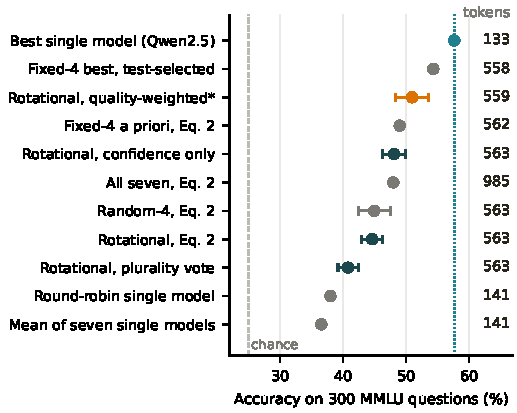
\includegraphics[width=\columnwidth]{figs/fig2_council.pdf}
\caption{Accuracy of single models and councils on the same 300 questions; bars show $\pm$1 SD over ten seeds, and the right column gives total tokens per query.}
\label{fig:council}
\end{figure}

The ablation isolates each part of the mechanism. Rotation itself adds no accuracy: rotational and random four-model councils differ by 0.4 points, well within their seed-to-seed spread. Its measurable effect is on load: over 300 queries no model waited more than 8 queries between selections under rotation, against 12 under random selection, while the spread of selection counts was the same (coefficient of variation 0.046 against 0.049). Within the consensus score, the agreement term is the harmful part. Agreement only (40.5\%) and plurality vote (40.8\%) are worse than confidence only (48.1\%), because the four near-chance models often agree on the same wrong option. Errors were only weakly correlated across models (mean pairwise correlation 0.16), and at least one of the seven models was right on 86.3\% of questions, so the information is in the pool; equal-weight agreement does not recover it. Weighting by held-out accuracy recovered part of the gap (51.0\%) but still lost to the best single model. This matches ensemble theory, in which voting helps when members are individually better than chance and comparably accurate \cite{dietterich2000ensemble}, and the finding that more calls can lower accuracy \cite{chen2024calls}.

\subsection{Deadlines and Member Failure}
Dropping members that miss a deadline bounds latency at the cost of accuracy. With the deadline set at the 90th percentile of single-call latency (2.19\,s), the council averaged 3.6 members, its 95th-percentile latency fell from 3.37\,s to 2.19\,s, and accuracy fell from 43.7\% to 42.7\% (seed 1); 4 of 300 queries returned no answer. A median deadline (1.37\,s) left two members on average, 54 unanswered queries and 33.7\% accuracy. When each member failed independently with probability 0.25 or 0.5, accuracy was 42.8\% and 39.7\% (10 seeds), so the council degrades gradually rather than failing outright.

\subsection{Adaptive Memory}
\textit{Task.} Because no public benchmark matches multi-session enterprise memory, a seeded synthetic task was built with fictional entities. Forty earlier sessions each left four memory entries (two project facts, such as a budget code, owner, hosting vendor or go-live date, and two routine remarks), giving 160 entries and about 2,100 prompt tokens of history. Test queries either ask for one stored fact (68 queries) or need no memory at all (32 arithmetic queries). Twenty further queries were held out to set $\tau$ before testing: $\tau$ was fixed at 0.22, the highest top-1 similarity of any memory-free calibration query plus a margin of 0.05. Qwen2.5-1.5B answered every query under four conditions (Table~\ref{tab:memory}), and an answer counted as correct when it contained the gold string.

\begin{table}[t]
\caption{Memory Conditions (Qwen2.5-1.5B; 68 Memory and 32 Memory-Free Queries)}
\label{tab:memory}
\centering
\footnotesize
\setlength{\tabcolsep}{3pt}
\begin{tabular}{@{}lccccc@{}}
\toprule
Condition & Mem. acc. & Free acc. & Tokens & Lat. (s) & Entries \\
\midrule
No memory & 0.0\% & 84.4\% & 44 & 1.39 & 0 \\
Full history & 79.4\% & 68.8\% & 2,137 & 29.56 & 160 \\
Fixed top-5 & 100\% & 62.5\% & 130 & 2.08 & 5 \\
Adaptive ($\tau$=0.22) & 100\% & 78.1\% & 102 & 1.67 & 3.4 \\
\bottomrule
\end{tabular}
\end{table}

\textit{Results.} Sending the full history cost 2,137 prompt tokens and 29.6\,s per query and still missed 14 of 68 stored facts (79.4\%, 95\% CI 69.1--88.2\%), all of which the adaptive condition answered ($p<0.001$); this is consistent with weaker use of facts buried in long contexts \cite{liu2024lost}. Both retrieval conditions found the gold entry for every memory query, but four of the five entries injected by fixed top-5 retrieval were not needed, and on memory-free queries those irrelevant notes lowered accuracy from 84.4\% to 62.5\%. Threshold gating kept memory out of 29 of the 32 memory-free queries, which recovered most of that loss (78.1\%; 7 gains and 2 losses against top-5, $p=0.18$) and cut mean prompt tokens by 21\% against top-5 and by 95\% against full history. A retrieval-only sweep showed that any $\tau$ from 0.30 to 0.60 would have excluded every memory-free query while keeping every gold entry; at 0.70, recall fell to 89.7\%. The calibrated value of 0.22 was therefore conservative. Each fact is phrased close to its query, so these numbers bound the token saving better than they predict accuracy on real records.

\subsection{Tool Access and Sensitive Data}
The gateway was checked in an earlier real MCP run on a workstation, using the official MCP Python SDK, a local Ollama runtime and three models (Qwen3 4B, Qwen3 8B and Llama 3.1 8B). Each model ran three scenarios against a server exposing a permitted \texttt{read\_status} tool and a high-risk \texttt{admin\_export} tool: an authorised read, a direct request to export data, and an injected instruction to export hidden in returned content. All three authorised reads succeeded. No export succeeded in the six adversarial runs. Two models attempted the direct export and the gateway rejected both calls as out of scope; the third declined. Under injection, no model attempted the export. These are nine single runs, and refusals reflect model behaviour as much as the gateway; the direct evidence for the gateway is the two denied calls, five passing authorisation unit tests, and a deterministic trace in which an out-of-scope export failed with \texttt{out\_of\_scope} and a call whose token belonged to another task failed with \texttt{task\_mismatch}.

\textit{Access control and sensitive data.} Persistent memory introduces risks that the token check does not cover. An attacker who can write a memory entry can plant an instruction that a later session retrieves \cite{greshake2023injection}, and memories can hold personal or regulated data. The design therefore stores the source session and writer with each entry, retrieves only within the requesting tenant and role, keeps retrieved text in a data channel, and lets retention rules exclude classes of data from storage or retrieval. Threshold gating also reduces exposure: in the memory experiment, queries that needed no memory received no stored entries. Tool-execution risk is limited by task-bound, short-lived tokens, by a least-privilege tool scope for each agent role and by supervisor approval for high-risk tools, following the excessive-agency and prompt-injection items of the OWASP list \cite{owasp2025}; the gateway logs every decision with its role, tool and task for audit. Attacks on the MCP layer itself, such as tool-description poisoning catalogued in MCPSecBench \cite{yang2025mcpsecbench}, were not tested here.

\subsection{Limitations}
The models are small (1--1.7 billion parameters) and uneven in quality, and the council results may differ for larger or more evenly matched pools. Only multiple-choice questions were tested, parallel latency is estimated from sequential calls on one CPU, and the council-size and strong-member analyses reuse the same 300 questions, so they are descriptive rather than held-out. The memory task is synthetic and was run with one model. The supervisor, the LangGraph orchestration, Kubernetes deployment, server-sent event (SSE) streaming and document parsing were not evaluated, and no claim is made about them. The harness, question identifiers, raw per-call logs and analysis scripts are published at \url{https://github.com/venumadhav0583/mcp-swarm} so that every number in this section can be recomputed.

\section{Conclusion}
This paper evaluated MCP-Swarm under a controlled design. Three findings change how the framework should be used. First, a council of small, uneven models did not beat its strongest member: the rotational council reached 44.6\% against 57.7\% for Qwen2.5-1.5B at four times the token cost, because near-chance models outvote the stronger ones. No council of any size from two to seven beat it, while tokens and CPU time grew with every member. Rotation added no accuracy over random selection; it bounded idle time. Confidence carried more signal than agreement, and accuracy-based weighting narrowed but did not close the gap. Second, threshold-gated memory was the clearest gain: it answered every stored-fact query at 5\% of the full-history token cost, where full history missed 21\% of facts, and it kept irrelevant memory out of most queries that needed none. Third, task-scoped tokens blocked every observed unauthorised export call in a small real MCP run. In practice, the council is worth its cost only when members are individually strong and comparably accurate, and member weights should come from held-out accuracy rather than equal votes. Future work will test larger pools, open-ended enterprise tasks and attacks on the MCP layer.

\begin{thebibliography}{99}
\bibitem{mcpspec} Anthropic, ``Model Context Protocol specification, version 2025-06-18,'' 2025. [Online]. Available: \url{https://modelcontextprotocol.io/specification/2025-06-18}
\bibitem{hou2025mcp} X. Hou, Y. Zhao, S. Wang, and H. Wang, ``Model Context Protocol (MCP): Landscape, security threats, and future research directions,'' arXiv:2503.23278, 2025.
\bibitem{guo2024survey} T. Guo, X. Chen, Y. Wang, R. Chang, S. Pei, N. V. Chawla, O. Wiest, and X. Zhang, ``Large language model based multi-agents: A survey of progress and challenges,'' in \textit{Proc. IJCAI}, 2024, pp. 8048--8057.
\bibitem{wu2023autogen} Q. Wu, G. Bansal, J. Zhang, Y. Wu, B. Li, E. Zhu, L. Jiang, X. Zhang, S. Zhang, J. Liu, A. H. Awadallah, R. W. White, D. Burger, and C. Wang, ``AutoGen: Enabling next-gen LLM applications via multi-agent conversation,'' arXiv:2308.08155, 2023.
\bibitem{li2023camel} G. Li, H. A. A. K. Hammoud, H. Itani, D. Khizbullin, and B. Ghanem, ``CAMEL: Communicative agents for `mind' exploration of large language model society,'' in \textit{Proc. NeurIPS}, 2023.
\bibitem{hong2023metagpt} S. Hong \textit{et al.}, ``MetaGPT: Meta programming for a multi-agent collaborative framework,'' in \textit{Proc. ICLR}, 2024.
\bibitem{cemri2025fail} M. Cemri \textit{et al.}, ``Why do multi-agent LLM systems fail?'' arXiv:2503.13657, 2025.
\bibitem{wang2023selfconsistency} X. Wang, J. Wei, D. Schuurmans, Q. Le, E. Chi, S. Narang, A. Chowdhery, and D. Zhou, ``Self-consistency improves chain of thought reasoning in language models,'' in \textit{Proc. ICLR}, 2023.
\bibitem{du2024debate} Y. Du, S. Li, A. Torralba, J. B. Tenenbaum, and I. Mordatch, ``Improving factuality and reasoning in language models through multiagent debate,'' in \textit{Proc. ICML}, 2024.
\bibitem{wang2024moa} J. Wang, J. Wang, B. Athiwaratkun, C. Zhang, and J. Zou, ``Mixture-of-Agents enhances large language model capabilities,'' arXiv:2406.04692, 2024.
\bibitem{jiang2023blender} D. Jiang, X. Ren, and B. Y. Lin, ``LLM-Blender: Ensembling large language models with pairwise ranking and generative fusion,'' in \textit{Proc. ACL}, 2023, pp. 14165--14178.
\bibitem{chen2024calls} L. Chen, J. Q. Davis, B. Hanin, P. Bailis, I. Stoica, M. Zaharia, and J. Zou, ``Are more LLM calls all you need? Towards scaling laws of compound inference systems,'' arXiv:2403.02419, 2024.
\bibitem{dietterich2000ensemble} T. G. Dietterich, ``Ensemble methods in machine learning,'' in \textit{Multiple Classifier Systems}, LNCS 1857. Berlin: Springer, 2000, pp. 1--15, doi: 10.1007/3-540-45014-9\_1.
\bibitem{lamport1982byzantine} L. Lamport, R. Shostak, and M. Pease, ``The Byzantine generals problem,'' \textit{ACM Trans. Program. Lang. Syst.}, vol. 4, no. 3, pp. 382--401, 1982, doi: 10.1145/357172.357176.
\bibitem{lewis2020rag} P. Lewis \textit{et al.}, ``Retrieval-augmented generation for knowledge-intensive NLP tasks,'' in \textit{Proc. NeurIPS}, 2020, pp. 9459--9474.
\bibitem{packer2023memgpt} C. Packer, S. Wooders, K. Lin, V. Fang, S. G. Patil, I. Stoica, and J. E. Gonzalez, ``MemGPT: Towards LLMs as operating systems,'' arXiv:2310.08560, 2023.
\bibitem{liu2024lost} N. F. Liu, K. Lin, J. Hewitt, A. Paranjape, M. Bevilacqua, F. Petroni, and P. Liang, ``Lost in the middle: How language models use long contexts,'' \textit{Trans. Assoc. Comput. Linguistics}, vol. 12, pp. 157--173, 2024, doi: 10.1162/tacl\_a\_00638.
\bibitem{reimers2019sbert} N. Reimers and I. Gurevych, ``Sentence-BERT: Sentence embeddings using Siamese BERT-networks,'' in \textit{Proc. EMNLP-IJCNLP}, 2019, pp. 3982--3992.
\bibitem{greshake2023injection} K. Greshake, S. Abdelnabi, S. Mishra, C. Endres, T. Holz, and M. Fritz, ``Not what you've signed up for: Compromising real-world LLM-integrated applications with indirect prompt injection,'' in \textit{Proc. 16th ACM Workshop Artif. Intell. Secur. (AISec)}, 2023, pp. 79--90, doi: 10.1145/3605764.3623985.
\bibitem{yang2025mcpsecbench} Y. Yang, C. Gao, D. Wu, Y. Chen \textit{et al.}, ``MCPSecBench: A systematic security benchmark and playground for testing Model Context Protocols,'' arXiv:2508.13220, 2025.
\bibitem{owasp2025} OWASP Foundation, ``OWASP Top 10 for LLM applications 2025,'' 2024. [Online]. Available: \url{https://genai.owasp.org/llm-top-10/}
\bibitem{langgraph} LangChain, ``LangGraph documentation,'' 2026. [Online]. Available: \url{https://docs.langchain.com/oss/python/langgraph/overview}
\bibitem{chroma} Chroma, ``Chroma documentation,'' 2026. [Online]. Available: \url{https://docs.trychroma.com/docs/overview/introduction}
\bibitem{hendrycks2021mmlu} D. Hendrycks, C. Burns, S. Basart, A. Zou, M. Mazeika, D. Song, and J. Steinhardt, ``Measuring massive multitask language understanding,'' in \textit{Proc. ICLR}, 2021.
\bibitem{llamacpp} G. Gerganov \textit{et al.}, ``llama.cpp: LLM inference in C/C++,'' 2026. [Online]. Available: \url{https://github.com/ggml-org/llama.cpp}
\end{thebibliography}

\end{document}
